\documentclass[../main.tex]{subfiles}
\begin{document}

\hypertarget{participants-and-design}{%
\subsection{Participants and design}\label{participants-and-design}}

Undergraduate and graduate phonetics and psychology students (80.8\%
female, median age = 21, IQR = 3, range = {[}18, 31{]}, total \(N\) =
207) participated in the study in exchange for course credit. We
employed a 2 (interpolated activity: episodic vs semantic recall) x 2
(feedback: given vs not given) between-subjects design. Rereading served
as a comparison interpolated activity, which was given to an additional
control group. In total, this amounts to five separate groups, to which
the participants were randomly assigned.

\hypertarget{materials-and-procedure}{%
\subsection{Materials and procedure}\label{materials-and-procedure}}

Participants read an expository text about weeds, drawn from a chapter
in a university-level textbook. Some sentences and passages were
slightly modified, so as to avoid odd language constructions; terms from
the binomial nomenclature were translated, and, taking into account the
characteristics of the target participant population, some plant names
were removed from the text to make it more approachable. The text was
divided into three interrelated parts (874, 754, and 835 words)
constituting an integrated body of knowledge. Additionally, a practice
text (768 words), not directly related to any of the other three parts,
was taken from the same chapter. The materials were presented on a PC,
in an application constructed using the open source \textit{oTree}
framework \citep[version 2.1.35,][]{chenOTreeOpensourcePlatform2016} for
the \textit{Python} programming language (version 3.6.4, October 20,
2018).

For the interpolated activity, participants either (i) answered ten
multiple choice questions related to the content of the part they have
previously read (episodic recall, hereafter referred to as
content-related testing), (ii) answered ten general knowledge multiple
choice questions (semantic recall, hereafter referred to as
general-knowledge testing) or (iii) reread the same part of the text
they have previously read.

Further, we manipulated whether or not participants received feedback on
their accomplishment on the interpolated tests. Feedback was presented
on a separate screen which listed the questions, the participant's
answers, and the correct answers in a tabular format. Incorrectly
answered questions were highlighted in red, and correctly answered
questions in green. After 40 seconds elapsed, a ``Next'' button
appeared, allowing participants to proceed to the next part. By setting
this cooldown period, by emphasising that there would be a cumulative
test, and through written instructions, we wanted to encourage our
participants to carefully examine the feedback. The feedback was
presented for maximally 60 seconds, after which the application
proceeded to the next part.

\begin{figure}[p]
  \centering
  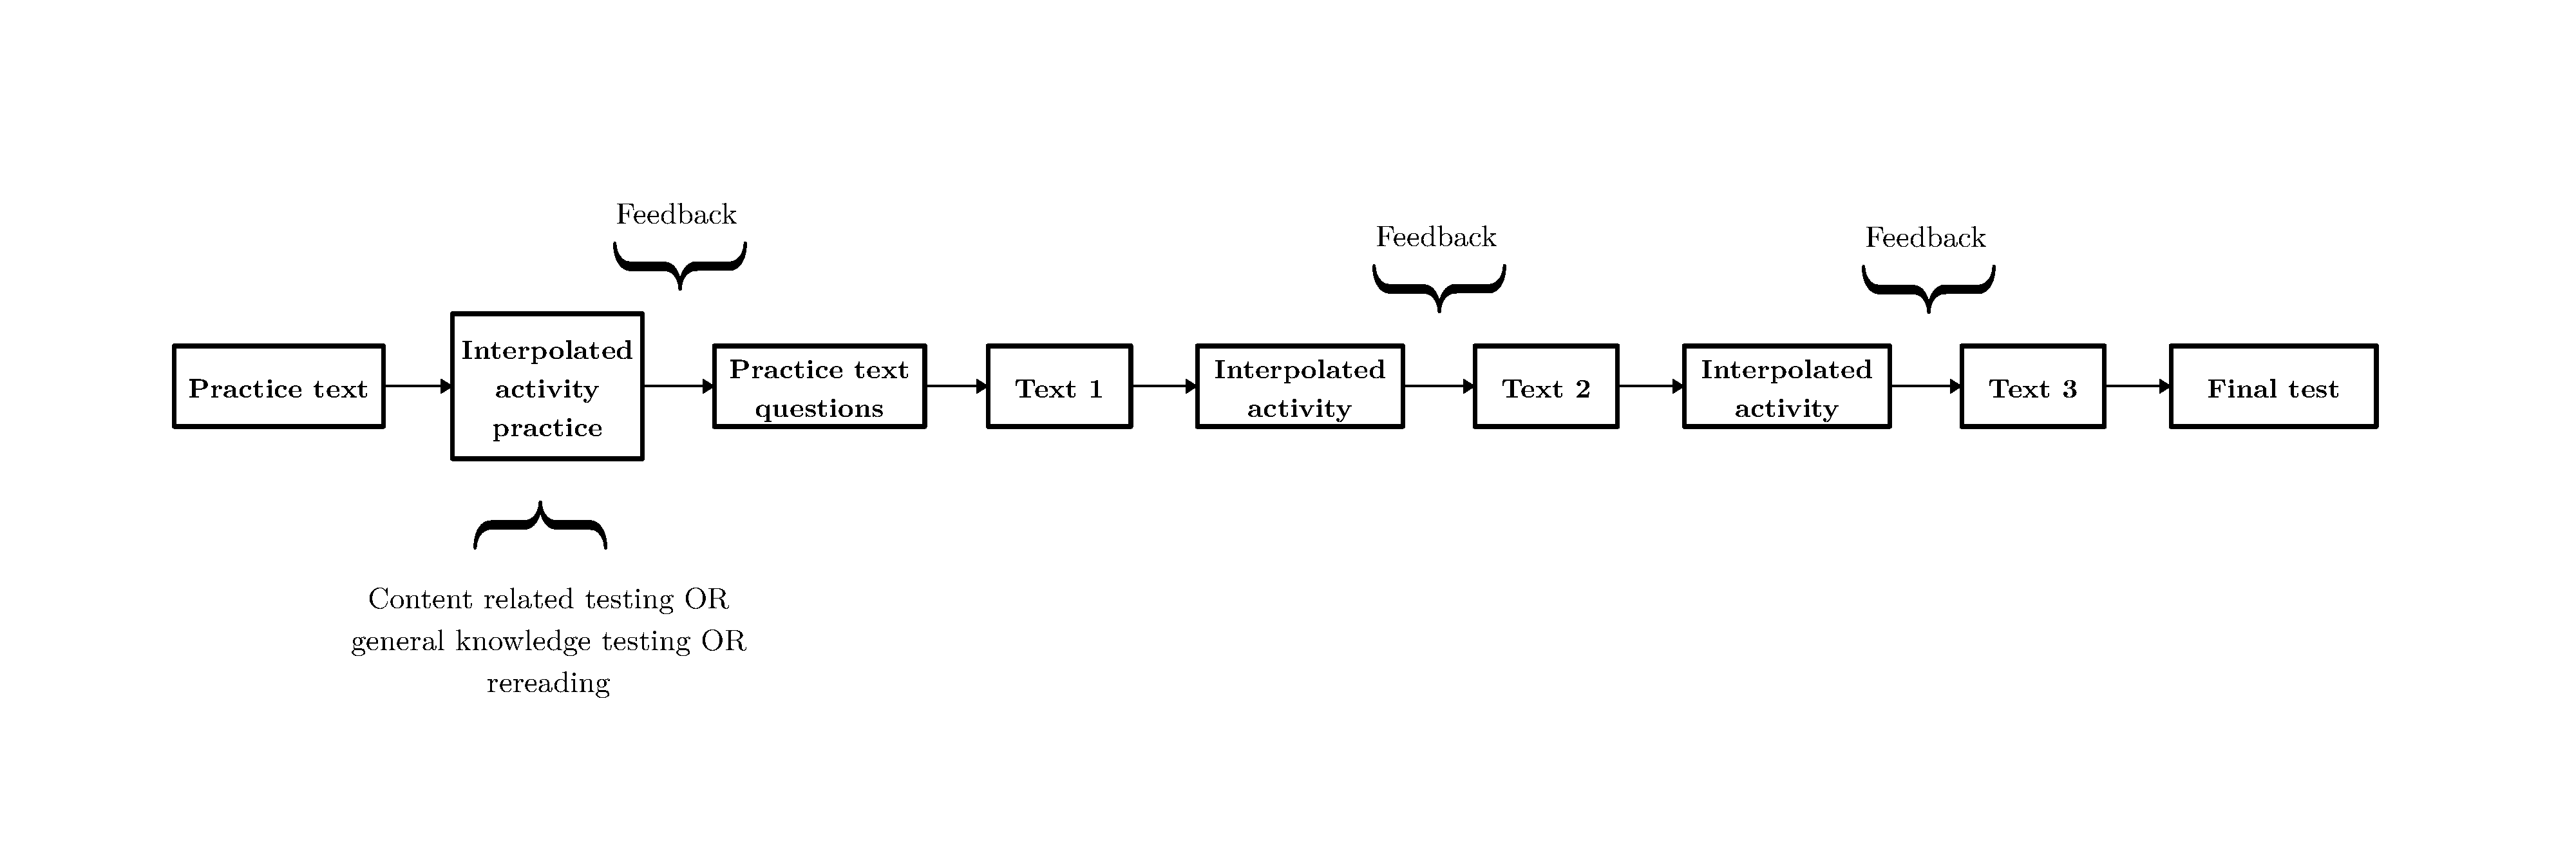
\includegraphics[width = 1.3\textwidth, keepaspectratio, angle = 90, trim = 0 0 0 0]{images/procedure.pdf}
  \caption{A flowchart depicting the experimental procedure.}
  \label{flowchart}
\end{figure}

The general procedure is shown in Figure \ref{flowchart}. Participants
were first given a brief introduction to the study, and were encouraged
to carefully read and follow the written instructions. Then, they were
led to a computer which was running a fullscreen instance of the
\textit{oTree} application with a randomly chosen experimental
condition. There, participants read the informed consent form and, in
case there were no questions, started the experiment.

After entering their personal information, participants were presented
with the instructions for their first task, which was to read the
practice text at a speed that comes naturally to them. Unbeknownst to
the participants, the time they took to read the practice text was
recorded, and used as the basis for determining the reading time limits
for the remaining texts. However, the lowest possible time limit was set
to 5 minutes, and the longest to 8 minutes.

Next, participants were familiarised with the interpolated activity they
were going to perform during the main part of the procedure. The
content-related test group answered four questions based on the practice
text, the general-knowledge test group answered four general knowledge
questions, and the rereading group reread the practice text (this time
with the time limit applied). Subjects in the rereading and general
knowledge conditions also answered the four questions related to the
practice text, in order to familiarise themselves with the scope and
specificity level of the questions they will receive after reading the
final text. Participants assigned to the feedback condition also
received feedback on their interpolated activity practice test
achievement.

After the practice round, participants proceeded to the main part of the
study, engaging in the interpolated activities they were assigned.
Depending on the condition they were assigned to, they also received
feedback after every interpolated test.

All participants were told that there would be a cumulative test after
the final part of the text, examining their knowledge of all three
parts. In reality, the final test examined only the knowledge of the
final part. Participants were presented with twenty questions examining
their knowledge of that part. No feedback was presented after the final
test, irrespective of the experimental condition. The computer recorded
whether a participant correctly answered a question and whether the
participant chose an intrusive distractor. This allowed us to compute
our dependent variables --- the total number of correct answers and the
total number of intrusive distractors chosen.

In total, forty-four content related questions with four response
options were generated from the presented parts of the text. Four
questions were presented after the practice text, ten after each of the
first two parts (only to the participants in the content related test
condition), and twenty after the third part of the text (to all
participants). Starting from the second ten-question-set, the distractor
options were chosen so that (a) two distractors were plausible, but
unrelated to the text, and (b) one distractor was a term or concept
mentioned in the previous part of the text --- this was considered to be
the ``intrusive'' distractor (sometimes reffered to as the ``intrusor''
in the rest of this article). Further, twenty-four general knowledge
questions were generated. These questions were presented to participants
in the general-knowledge test condition, after the first two parts of
the text and after the practice text.


\end{document}
